%\section{Probing hadronic acceleration sources}
%In this section one will look at different observables and methods of probing extra galactic sources as potential candidates for the origin of the UHECRs and/or neutrinos. The goal is to constrain our list of candidates by applying known effects and theoretical models to observed data. In brief one will be discussing, The hillas criterion, the anisotropy of the UHECRs and neutrinoes, "the emissivity of our sources in UHECRs and neutrinos", and a comprehensive time scale analysis of the sources.
This section outlines some different methods and observables used to probe hadronic accelerators as potential candidates for the origin of the UHECRs and/or neutrinos. The goal is to constrain our list of candidates by applying known effects and theoretical models to observed data, and to discuss the implications of these constraints. In brief, we will be discussing the density of sources, the spectral energy distribution, the magnetic field constraints, and a time scale analysis used to estimate the maximum energy attainable by ions.

\section{Density of sources}
\label{sec:prevalence_of_sources}

Due to the seemingly isotropic distribution of extra-galactic UHECRs, especially at semi-low energies as discussed in section \ref{sec:high_energy_particles} one can put limits on the density of sources. In \cite{ThePierreAugercollaboration_2013} they quote a density larger than $(0.06-5) 10^{-4} \rm{Mpc^{-3}}$ at a $95\% $ confidence level. This density, although not exceedingly large, would still dampen the idea of singular but powerful sources. Therefore, for any source to be considered, one needs to consider its density as well. 

To calculate the density of sources in the Universe there are several methods. The most common method for sources such as AGN is to use the luminosity function (LF) of the source.
The luminosity function is a function that describes the number of sources per unit volume and luminosity. Typically, the focus is on the differential luminosity function, which is defined as
\begin{equation}
    \frac{d\Psi(L,z)}{dL} = \frac{d^2N(L,V_c(z))}{dLdV_c(z)}.
\end{equation}

One also can change the differential of the comoving volume into a term only depending on the redshift assuming the source population is spread isotropically and by multiplying with the differential comoving volume element. This 
transformation goes as follows, 

\begin{equation}
    \frac{d^2N(L,V_c(z))}{dLdV_c(z)}\frac{dV_c(z)}{dz} = \frac{N(L,z)}{dLdz}.
\end{equation}

To effectively determine the LF, it's typical to divide it into two distinct components: a local term and a time evolution term.
This approach involves taking the local luminosity function, calculated at a redshift 
$z=0$, and then scaling it with a function that accounts for the change in redshift. 
The exact form of the total LF varies based on the source object, but it generally falls into two categories derived from the method of incorporating the growth term into the local LF.
These methods are selected based on which best represents the observed evolution.

The two distinctions are the Pure Density Evolution (PDE) and the Pure Luminosity Evolution (PLE). 
The PDE model modifies the local density function to reflect changes over time, 
while the PLE model adjusts the local luminosity. The evolution is better represented by their equations and is given as 

\begin{equation}
\frac{d\Psi(L,z)}{d(L)} = 
    \begin{cases}
        \frac{d\Psi(L/e(z),z=0)}{d(L)} \quad (PLE)\\
        \frac{d\Psi(L,z=0)}{d(L)}e(z) \quad (PDE)\\
    \end{cases} .
\end{equation}

For some sources which lack observational data, it can be difficult to estimate a full luminosity function. Due to the lack of observation or a big bias in the catalogue selection, different sources are not constrained enough and therefore one must rely on simpler estimates of their densities. One such method given that the lifetime of a source is known is via probability. The density is estimated by calculating the required density one needs to produce the observed amount of sources, or in the worst case one source given its average lifetime. This will in most cases serve as a lower limit, and give us a starting point for further analysis.  

In order to do so, one defines the probability of seeing a source that has a lifetime $t_l $ up to a horizon $t(z)$ as 

\begin{equation}
    p = \frac{t_l}{t(z)}.
\end{equation}
The horizon is the redshift at which one stops finding appreciable number of the source. The required density such that one observes a source at present time can then be estimated as 

\begin{equation}
    n = \frac{1}{p V(z)} 
\end{equation}

Where $V(z)$ is the comoving volume of the Universe up to the horizon.
The calculation is crude, but allows us to make lower limit estimates on sources where the Luminosity function is not defined. An example of this is seen in section \ref{sec:prevalence} where we estimate the density of CSOs.


\section{SED broad band analysis}
The spectral shape of emitting galaxies and galaxy cores tells us a lot about the underlying dynamics, and with this information we can start to peel away the complex layers. The spectral energy distribution (SED) of a source is a plot of the photon energy emitted by the source as a function of frequency. In Figure \ref{fig:AGN_SED} one can see a model of a typical SED of an AGN in which the jet components, that is to say the synchrotron and inverse Compton components, are not dominant. The different components of the AGN are visible in the plot, and understanding how different components are created and contribute to the nearby environment will give us a better understanding of what observables we might expect from sources such as these. The following section will outline the different components of the SED and how they are modelled.

\begin{figure}
    \centering
    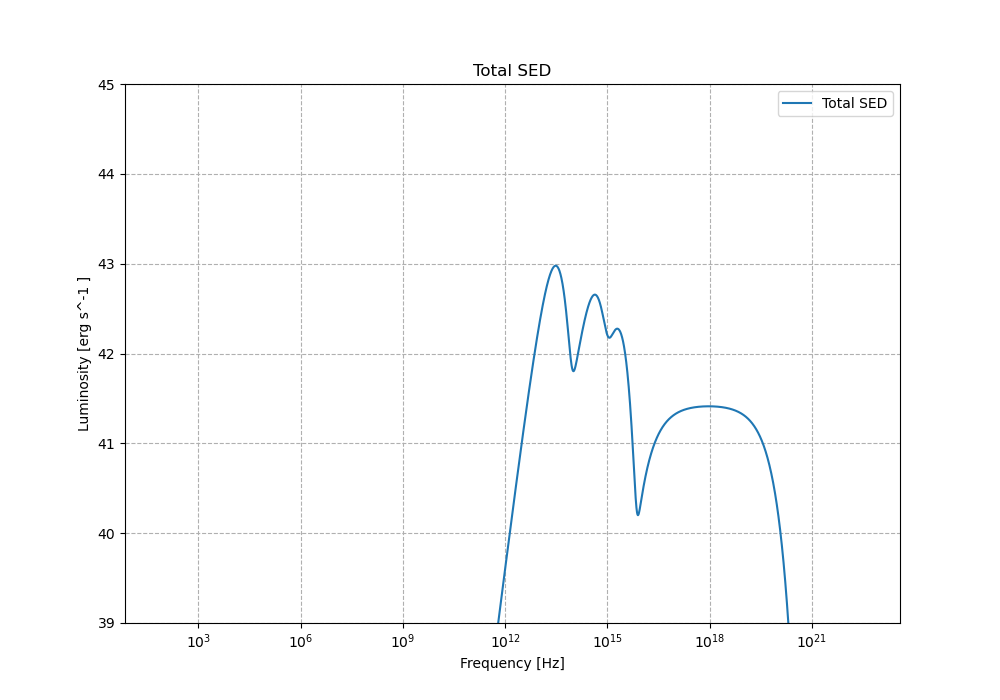
\includegraphics[width=0.9\textwidth]{C:/Users/henri/OneDrive/Documents/NTNU/Semester 10/Masteroppgave/Plots/SED.png}
    \caption{The spectral energy distribution of an AGN viewed without beaming from the jet. The different components of the AGN are visible in the plot.}
    \label{fig:AGN_SED}
\end{figure}

%\subsection{X-ray energy budget}
%The X-ray energy budget of especially Active galactic nuclei is often used as a probe for UHECRs and neutrino emissivity. This makes the X-ray Luminosity of AGN an interesting parameter that warrants further analysis. In this sense the X-ray luminosity is often used a proxy for the total energy budget of escaping particles, but a true relation between the two is not known. The X-ray luminosity of an AGN usually has two sources of emission, the corona, and IC scattering of the synchrotron radiation in the jets. In both cases the main mechanism is thought to be Inverse Compton scattering and for that one requires relativistic electrons. Requiring relativistic electrons is a good indicator that there might be relativistic protons present as well, and following that logic one can start to estimate the energy budget of the protons. 

%\subsection{Radio luminosity}
\subsection{Core photon fields around AGN}
\label{sec:photon_fields}

In order to determine the photon fields around AGN cores we follow \cite{Ghisellini_2009} which describes the photon fields surrounding a Blazar. The photon fields separate into different contributions from the different regions of a classic AGN as discussed in section \ref{sec:AGN}. 
The different core regions of an AGN are the accretion disk, the broad line region, the torus, and the X-ray corona. 

\textbf{Accretion disk:} The photon field emerging from an accretion disk is calculated by assuming a black body spectrum at each ring of a Shakura-Sunyaev disk and summing up its contributions. The temperature of 
each ring in the disk is given by 

\begin{equation}
    T(R) = \left(\frac{3 R_{S} L_{d}}{16 \pi R^3 \eta \sigma_{\mathrm{SB}}} \left(1-\left(\frac{3 R_{S}}{R}\right)^{\frac{1}{2}}\right) \right)^{\frac{1}{4}}
\end{equation}

Each ring of the accretion disk is assumed to be emitting as a black-body spectrum, which is defined as

\begin{equation}
    \label{eq:BB}
    I(\nu) = \frac{2 h \nu^3}{c^2} \left(\frac{1}{\exp\left(\frac{h \nu}{k_B T}\right) - 1}\right).
\end{equation}

By integrating the intensity over all annuli of the disk we can find the total flux of the disk and from there the total energy density of the disk per frequency.

The resulting spectral energy density as seen in the comoving frame of an observer at $R$ is then given by

\begin{equation}
    u_d'(\nu') = \frac{2\pi}{c} \int_{\mu_d}^1 I'(\nu')\delta^{-2} d\mu
\end{equation}
where $\mu_d$ is the cosine of the angle between the location on the disk and the normal of the disk with respect to the observer, and $\delta = \Gamma(1-\beta \mu)$ is the Doppler factor. 

\textbf{X-ray corona:} The photon field from the X-ray corona is assumed to be a power law spectrum with a cut off at high energies. Its total energy emitted is related to the disk luminosity 
by the equation $L_{cor} = f_X L_d$ where $f_X$ is the fraction of the disk luminosity that is emitted by the corona. The spectral energy density of the corona is then given by 

\begin{equation}
    U_{cor}(\nu) = D(R)\left(\frac{\nu}{\nu_0}\right)^{-\alpha} \exp\left(-\frac{\nu}{\nu_{cut}}\right)
\end{equation}

The factor $D(R)$ is a scaling factor that incorporates the position of the observer. The integral of the spectral energy density over all frequencies should equate to the total energy density in X-ray at the location of the observer.

The energy density of X-ray around the central engine is given by

\begin{equation}
    \text{UX'}(R) = \frac{f_{X} L_{d} \Gamma^2}{\pi (R_{X})^2 c} \left(1 - \mu_{X} - \beta(1 - \mu_{X}^2) + \frac{\beta^2 (1 - \mu_{X}^3)}{3}\right)
\end{equation}
where
\[
\mu_{X} = \left(1 + \frac{R_{X}^2}{R^2}\right)^{-0.5}.
\]

Here $f_{X}$ is the fraction of the disk luminosity that is emitted by the X-ray corona, $L_{d}$ is the disk luminosity, $\Gamma$ is the Lorentz factor of the jet, $R_{X}$ is the size of the X-ray corona, $\beta$ is the velocity of the observer in units of the speed of light.
In short, the X-ray energy density stays constant until the observer is further away where it will decrease as $1/R^2$ which is to be expected.

\textbf{Broad line region:} The broad band field is assumed to be emitting a black body spectrum as in equation \ref{eq:BB} which peaks at the Lyman-alpha line. The Lyman-alpha line is a spectral line of hydrogen when the atomic electron transitions from the $n=2$ to the $n=1$ orbital.
Similarly to the X-ray corona, the spectral energy density is scaled to the region of interest and the total energy density as a function of distance is given by: 

\begin{equation}
    \label{eq:UBLR}
    \text{UBLR'}(R) = 
    \begin{cases}
    \frac{17}{12}\frac{f_{\text{BLR}} L_{d} \Gamma^2}{4\pi R_{\text{BLR}}^2 c} & \text{if } R \leq R_{\text{BLR}}, \\
    \frac{f_{\text{BLR}} L_{d} \Gamma^2}{4 \pi R_{\text{BLR}}^2 c \beta 3} \left[2 (1 - \beta \mu_{\text{IR1}})^3 - (1 - \beta \mu_{\text{IR2}})^3 - (1 - \beta)^3\right] & \text{if } R \geq 3R_{\text{BLR}}, \\
    a R^b & \text{otherwise},
    \end{cases}  
\end{equation}
where 
\begin{align*}
    \mu_{\text{IR1}} &= \left(1 + \frac{R_{\text{BLR}}^2}{R^2}\right)^{-0.5}, \\
    \mu_{\text{IR2}} &= \left(1 - \frac{R_{\text{BLR}}^2}{R^2}\right)^{-0.5}, \\
    %b &= \log\left(\frac{\text{UBLR}(3R_{\text{BLR}}, R_{\text{BLR}}, f_{\text{BLR}}, L_{d}, \Gamma)}{\text{UBLR}(R_{\text{BLR}}, R_{\text{BLR}}, f_{\text{BLR}}, L_{d}, \Gamma)}\right) / \log(3), \\
    %a &= \frac{\text{UBLR}(R_{\text{BLR}}, R_{\text{BLR}}, f_{\text{BLR}}, L_{d}, \Gamma)}{R_{\text{BLR}}^b}.
\end{align*}

\textbf{Torus:} There is also assumed to be a dusty torus around the AGN emitting in infrared. The spectral energy density of the torus is also given by 
a black body spectrum given in equation \ref{eq:BB}. The total energy density of the torus has the same relations 
as the BLR for $R>R_{IR}$ but with the relevant parameters for the torus. For $R<R_{IR}$ the energy density is given as

\begin{equation}
    \text{UIR'}(R) = 
    \begin{cases}
    \frac{f_{\text{IR}}L_d \Gamma^2}{4 \pi R_{\text{IR}}^2 c} & \text{if } R \leq R_{\text{IR}}, \\
    \end{cases}
\end{equation}

\subsection{Non-core photon fields}
\label{sec:non_core_photon_fields}
In addition to the core photon fields we will model the photon field from relativistic electrons occupying a magnetic field, i.e. Synchrotron radiation, Synchrotron self Compton radiation, and Inverse Compton radiation of the core fields. The information and derivation of these subsections are taken from \cite{BHradiation}. We note lastly that all calculations below are done in the comoving frame of the source, and one must transform the results to the observer frame if one wishes to estimate observed flux quantities.

\begin{figure}
    \centering
    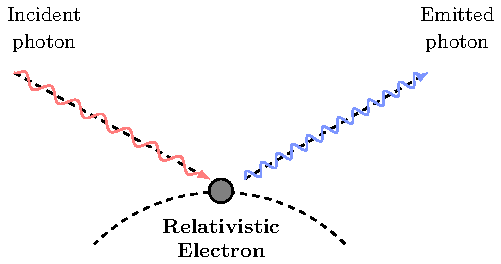
\includegraphics[width=0.7\textwidth]{C:/Users/henri/OneDrive/Documents/NTNU/Semester 10/Masteroppgave/Plots/Inverse_compton.pdf}
    \caption{The inverse Compton scattering process. The process is the scattering of a low energy photon by a relativistic electron. The scattered photon will have a higher energy than the original photon. Image taken from \cite{BennumAlfred}}
\end{figure}

\textbf{Synchrotron radiation:} 
\label{sec:synchrotron_radiation}
For a given population of relativistic electrons that occupy energies between $\gamma_{min}$ and $\gamma_{max}$ in a magnetic field $B$, the movement of the electrons through the magnetic field will cause them to spiral, and in turn emit synchrotron radiation. For relativistic particles at pitch angle $\pi/2$ to the magnetic field, the spectral energy radiated per revolution at $\omega = 2\pi \nu$ around the magnetic field is given by

\begin{equation}
    I(\omega) = \frac{2 e^2 \omega}{\sqrt{3}\gamma^2 \omega_L c} \int_{2\omega/3\omega_L\gamma^2 }^{\infty} K_{5/3}(\xi)d\xi  
\end{equation}

where $\omega_L = eB/mc$ is the Larmor frequency.

The radiated power at the frequency $\nu$ is $P(\nu) = 2\pi P(\omega) = \omega_L I(\omega)$ which allows us to write the power radiated by an electron at frequency $\nu$ as

\begin{equation}
    P(\nu) = \frac{\sqrt{3} e^3 B}{m c^2} \left(\frac{\nu}{\nu_c}\right) \int_{\nu/\nu_c}^{\infty} K_{5/3}(\xi)d\xi = \frac{\sqrt{3} e^3 B}{m c^2} F\left(\frac{\nu}{\nu_c}\right)
\end{equation}

where $\nu_c = \frac{3\gamma^2}{2}\left(\frac{eB}{2\pi m_e c}\right)$ is the critical frequency.

We will now skip a few steps for brevity, but if one is interested, one can find the full derivation in \cite{BHradiation} on page 126. Then for a distribution $N(\gamma)$ of electrons where the average distribution of electrons is static, and averaged over all pitch angles we can write the total power radiated as

\begin{equation}
    P(\nu) = \frac{\sqrt{3} e^3 B}{m c^2} \int_{\gamma_{min}}^{\gamma_{max}} N(\gamma) R\left(\frac{\nu}{\nu_c}\right)d\gamma
\end{equation}

where 

$$
R(\nu/\nu_c = x) =  \frac{x}{2} \int_0^\pi d\theta \sin\theta \int_{x/\sin(\theta)}^{\infty} K_{5/3}(t)dt
$$
\begin{equation}
    = \frac{1}{2}\pi x(W_{0,\frac{4}{3}}(x)W_{0,\frac{1}{3}}(x)-W_{\frac{1}{2},\frac{5}{6}}(x)W_{\frac{-1}{2},\frac{5}{6}}(x))
\end{equation}
Here the $W$ functions are the Whittaker functions, these are defined in the appendix. 

In addition to emitting synchrotron radiation, the same electrons can also absorb the radiation. This is called synchrotron self-absorption, and the relation between the full synchrotron power and the observed synchrotron power for a sphere due to self-absorption is

\begin{equation}
P(\nu)_{\text{SSA}} = P(\nu)_{\text{syn}}\frac{3 u(\tau_{\nu})}{\tau_{\nu}}
\end{equation}
where $\tau_{\nu} = 2 \kappa_{\nu} r_b$ is the frequency-dependent optical depth, and 
$u(\tau_{\nu}) = \frac{1}{2}\left(1- \frac{2}{\tau^2}[1-(1+\tau)\exp{-\tau}]\right)$. The parameter of interest is the frequency-dependent self-absorption coefficient $\kappa_{\nu}$ which can be estimated via a delta approximation as 

\begin{equation}
    \kappa_{\nu, approx} = -\frac{\pi}{36} \cdot \frac{c r_e}{\nu} \left[\gamma^2 \frac{d}{d\gamma}\left(\frac{n(\gamma)}{\gamma^2}\right) \right]_{\gamma = \sqrt{\frac{\nu}{2 \nu_B}}}
\end{equation}

where $\nu_B = \frac{e B}{2 \pi m_e c }$ is the critical frequency of the magnetic field.

\textbf{Synchrotron self Compton radiation:}
In addition to radiating synchrotron radiation, non-thermal electrons also have the ability to Compton scatter on the same radiation that they emit. This radiation is called synchrotron self Compton radiation (SSC). In order to calculate the resulting radiation, We must first calculate the energy density of the synchrotron radiation. For a given sphere of emitting electrons, the average energy density of the synchrotron radiation is given as

$ u(\nu) = \frac{1}{4 \pi R^2 c} P(\nu) $
    
We again skip some steps and define the SSC luminosity as

\begin{equation}    
\epsilon_s J_{\text{SSC}}(\epsilon_s) =  \frac{3}{4} \sigma_T c \epsilon_s^2 \int_0^{\infty} d\epsilon \frac{u_{\text{syn}}(\epsilon)}{\epsilon^2} \int_{\gamma_{min}}^{\gamma_{max}} d\gamma \frac{N_e(\gamma)}{\gamma^2} F_C(q,\Gamma)
\end{equation}

where $\sigma_T$ is the Thomson cross section, $\epsilon_s$ is the energy of the SSC photon in dimensionless units: $\epsilon = \frac{h\nu}{m_e c^2}$, $u_{\text{syn}}$ is the energy density of the synchrotron radiation, $N_e$ is the electron distribution, and 

$$
F_c = \left(2q\ln (q) + (1+2q)(1-q) + \frac{1}{2}\frac{\Gamma q}{1+ \Gamma q}(1-q)\right)\times H\left(q; \frac{1}{4\gamma^2},1\right),
$$
$$
q = \frac{\epsilon_s}{\gamma \Gamma(1-\epsilon_s/\gamma)}, \quad \Gamma = 4\gamma \epsilon
$$

\textbf{Inverse Compton radiation:}

The last photon field to study is the inverse Compton radiation, which is similar to the SSC radiation but instead of scattering on the synchrotron radiation, the electrons scatter on the photon fields from the core. The biggest difference here is the angular dependency on the incoming photon field. For SSC we assumed that the synchrotron radiation was isotropic, but for IC we must take into account that the radiation comes from a narrow angle. For simplicity, we assumes that the external photon density follows this distribution 

\begin{equation}
    u_{ext}(\epsilon,\theta) = K u_{ext}(\epsilon)(1-\cos \theta)^4  
\end{equation}

where $K$ is a normalization constant. We then give the luminosity of the IC radiation as

\begin{equation}
    \epsilon_s J_{\epsilon}^{\text{EC}} = c \pi r_e^2 \epsilon_s^2 \int d\Omega \int_0^{\epsilon_{ext}^{\text{high}}} d\epsilon_{ext} \frac{u_{ext}(\epsilon_{ext}, \Omega)}{\epsilon{_ext}^2} \int_{\gamma_{\text{low}}}^{\infty} d\gamma \frac{N_e'(\gamma)}{\gamma^2} \Xi_C.
\end{equation}

where $r_e$ is the classical electron radius, $\epsilon_s$ is the energy of the IC photon, $u_{ext}$ is the energy

\section{Magnetic field constraints}
For acceleration in astrophysical sources one usually requires a relatively strong magnetic field. In this section, we will outline some methods for estimating the magnetic field strength in astrophysical sources based on their radio observations, namely the equipartition method and the synchrotron self-absorption method.

\subsection{Equipartition}
\label{sec:equipartition}
The most well-known estimate for magnetic field strength in astrophysical sources is through the equipartition argument. The fact that we observes synchrotron radiation implies that a source of relativistic electrons with energy density $U_e$ 
possess a magnetic field with energy density $U_B$. The question that one aims to answer with the equipartition argument is what is the minimum total energy in both relativistic particles and magnetic fields required to produce the observed synchrotron radiation of a given frequency. The total energy in relativistic particles and magnetic fields of a volume $V$ is given as

\begin{equation}
    U_{tot} = U_p + U_B = V(u_p + u_{mag})
\end{equation}

Here $u_p$ is the energy density of all relativistic particles, i.e., electrons, protons, and heavier ions ($Z>1$). Ions emit very little synchrotron radiation for a given energy $E$ compared to electrons, so little is known about their energy density; therefore, it is common to assume

\begin{equation}
    u_p = \eta u_e
\end{equation}

where $\eta$ is a constant $>1$ and $u_e$ is the energy density of the relativistic electrons. In order to estimate the energy density of the electrons, we assumes their distribution as a power law $n(E) \propto E^{-\delta}$, and their energy density becomes

\begin{equation}
    u_e = \int_{E_{min}}^{E_{max}} n(E) E dE = K \int_{E_{min}}^{E_{max}} E^{1-\delta }dE
\end{equation}

The radiated power of an electron peaks strongly around the critical frequency $\nu_c$, and following \cite{2013Wilson} Chapters 10.8 and 10.10, we can then write a relation between a frequency $\nu$ and energy $E$ as

\begin{equation}
    \nu = \frac{3}{2}\frac{eB}{m_e^3 c^5}E^2.
\end{equation}

This allows for the particle energy density to be written as

\begin{equation}
    \label{eq:energy_density_particles}
    u_p = K \frac{\eta}{1-2n} \left(\frac{e}{m^3c^5}\right)^{n-1/2}\left(\nu_{max}^{1/2-n}-\nu_{min}^{1/2-n}\right) B^{n-1/2} = K G B^{n-1/2}
\end{equation}
by introducing the constant $n = \frac{1}{2}(\delta -1 )$. 

The energy density of the magnetic field is given as

\begin{equation}
    u_{mag} = \frac{B^2}{8\pi}
\end{equation}

To move further, one wishes to eliminate the factor $K$ from our equations and relate it to observed properties. \cite{2013Wilson} gives the emissivity of a synchrotron source for tangled magnetic fields as

\begin{equation}
    \epsilon(\nu) = b(n)K \frac{e^3}{m c^2}\left[\frac{3 e}{4 \pi m^3 c^5}\right]^{n} B^{n+1} \nu^{-n} = H K B^{n+1} \nu^{-n},
\end{equation}

where $b(n)$ is a function of the spectral index $n$ given in the appendix. The observed flux density of a source with volume $V$ and at distance $R$ is given as

\begin{equation}
    \label{eq:flux_density_eq}
    S(\nu) = \frac{V}{R^2} \epsilon(\nu) \propto B^{n+1} \nu^{-n}
\end{equation}

Using this relation, we can then write the total energy density while inserting equation \ref{eq:flux_density_eq} as $K$ in equation \ref{eq:energy_density_particles} as

\begin{equation}
    U_{tot} = \frac{G}{H}R^2(S_v\nu^n)B^{-3/2} + \frac{V B^2}{8\pi}
\end{equation}

One then argues that $U_{tot}$ should have a minimum value, and given that we has measurements on distance, volume, and flux density, we can then estimate the magnetic field strength. The magnetic field strength will then be

\begin{equation}
    B_{eq} = \left(\frac{6\pi G}{H}\frac{R^2}{V}S_\nu \nu^n\right)^{2/7}
\end{equation}
This relationship between $U_B$ and $U_e$ at this minimum is very near the equipartition value, which is why this method is often called as such.


\subsection{Synchrotron self absorption}
\label{sec:SSA}

The theory of synchrotron self-absorption is a tool used previously for estimating magnetic field strength in spherically symmetric synchrotron sources. Synchrotron self-absorption is the process where the synchrotron radiation is absorbed by the same electrons that produced it as seen in section \ref{sec:synchrotron_radiation}, and the effect of this is that any given volume of emitting plasma that radiates synchrotron radiation will have a frequency below which the plasma is opaque. This frequency at which this happens is called the turnover frequency, and one aims to show how one can estimate the magnetic field strength in the emitting plasma based on this shape of the spectrum at this frequency. The concept was first introduced by \cite{1983ApJ...264..296M}, but this section relies heavily on \cite{Hirotani_2005} for the derivation. 

%Before we begin the derivation it is fitting to understand the spectrum of synchrotron radiation from a plasma. The spectrum is characterized by the peak frequency, also called the turnover frequency $\nu_m$, the peak flux density $S_m$, and naturally the spectral index $\alpha$. One referse the reader to image \ref{fig:synchrotron_spectrum} for a simple view of the synchrotron speaktrum in question. 

\begin{figure}
    \centering
    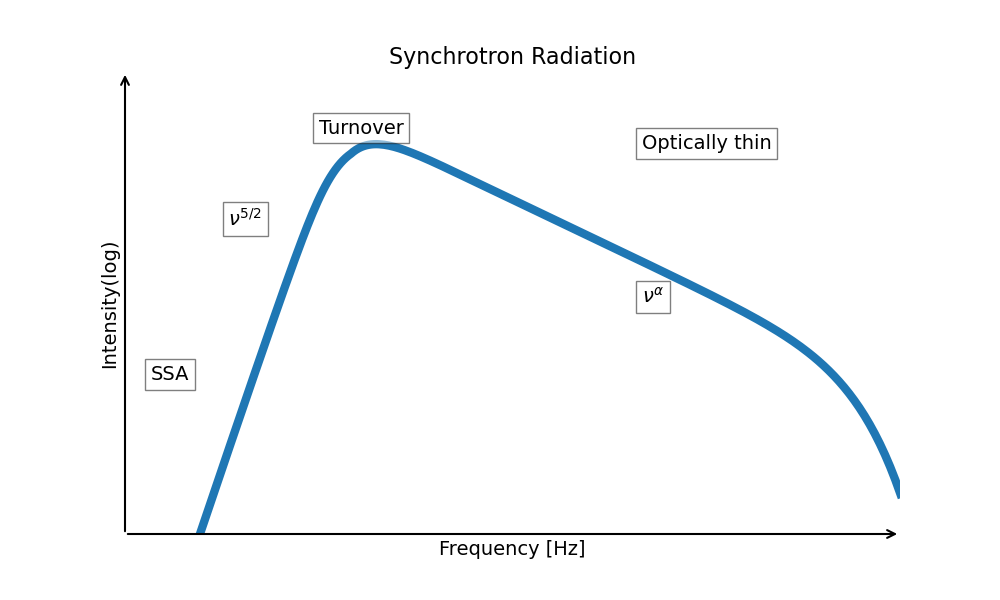
\includegraphics[width=0.75\textwidth]{C:/Users/henri/OneDrive/Documents/NTNU/Semester 10/Masteroppgave/Plots/Synchrotron_radiation.png}
    \caption{Typical synchrotron spectrum of a Giga hertz peaked galaxy (GHP). Later on we will see that GHP galaxies and CSO occupy the same niche. Image similar to one from Group of Active Galactic Nuclei investigation at https://www.sao.ru/hq/giag/gps-en.html }
    \label{fig:synchrotron_spectrum}
\end{figure}

In order to estimate the magnetic field strength we must assume that it is uniform and that the electron density is also uniform. From here the transfer equation for escaping synchrotron radiation is given in \cite{Hirotani_2005} and the specific intensity can be written as 

\begin{equation}
    I_\nu = A(\alpha) \nu^{'\frac{5}{2}}[1-\exp(-\alpha_{\nu}'x_0' )] 
\end{equation}
where 

\begin{equation}
    A(\alpha) = \frac{3}{2}^{-\alpha}\frac{e}{c}\frac{a(\alpha)}{C(\alpha)}\left(\frac{e}{2\pi m_e c}\right)^{-3/2}B^{-1/2}
\end{equation}

where $x_0'$ is the thickness of the emitting plasma along the observer's line of sight. The coefficients $a(\alpha)$ and $C(\alpha)$ are tabulated values that depend on the spectral index $\alpha$, not to be confused with the absorption coefficient $\alpha_{\nu}$, and any value denoted with a $'$ is in the comoving frame. 

Imagining an observer at a distance $D$ with angle $\theta$ from the blob of plasma (as seen in Figure \ref{fig:Radiative_transfer}), one can define the fractional thickness, which is a Lorentz-invariant quantity, as

\begin{equation}
    \frac{x_0'}{2R'} = \cos(\theta + \xi) = \sqrt{1-\left[\frac{\sin(\theta)}{\sin(\theta_d/2)}\right]^2}
\end{equation}

Determining that $\tau(0) \equiv  \alpha'2R'$ is the optical depth for $\theta = 0$, one can then get the full specific intensity as

\begin{equation}
    I_\nu(\theta) = \left( \frac{\delta}{1+z}\right)A(\alpha)\nu^{\frac{5}{2}}\left(1-\exp \left(-\tau(0)\sqrt{1-\left[\frac{\sin(\theta)}{\sin(\theta_d/2)}\right]^2}\right)\right)
\end{equation}

The shape of the blob is assumed to be spherical, and one can integrate the specific intensity over the entire blob to get the total flux density as

\begin{equation}
    \label{eq:flux_density}
    S_\nu = 2\pi \int_0^{\theta_d/2} I_v(\theta)\cos(\theta)\sin(\theta) = \pi \sin^2(\frac{\theta_d}{2})(\frac{\delta}{1+z})^{1/2}A \nu^{5/2} \int_0^1[1-\exp(-\tau(0)\sqrt{1-x^2})]dx
\end{equation}
where $x \equiv \left[\frac{\sin(\theta)}{\sin(\theta_d/2)}\right]^2$.
Here we insert what we know about the synchrotron spectrum and the turnover frequency $\nu_m$, notably that the derivative is zero at $\nu_m$. We derive the flux density with respect to frequency and set it equal to zero to find the equation that relates $\tau_\nu(0)$ and $\alpha$ at the turnover frequency. In order to do this, one needs to know the relation between the absorption coefficient and frequency. This is given also in \cite{Hirotani_2005} as 
\begin{equation}
    \alpha_\nu' = C(\alpha) r_e^2 k_e^*\frac{\nu_0}{\nu'}(\frac{\nu_B}{\nu'})^{(-2\alpha +3)/2}
\end{equation} 

where $\nu_e \equiv c/r_e$ is the electron frequency, $r_e \equiv e^2/(m_e c^2)$, and  
$\nu_B \equiv eB/(2\pi m_e c)$ is the cyclotron frequency. 

Having the solution for $\tau_\nu(0)$ as a function of $\alpha$, we denotes the solution at the turnover frequency as $\tau_m(0)$. This is a tabulated value and the table from \cite{Hirotani_2005} is found in the appendix.

Using this solution, we can inversely solve equation \ref{eq:flux_density} for the magnetic field strength $B$ and obtain with the small angle approximation 

\begin{equation}
    B =   10^{-5} b(\alpha) \left(\frac{S_m}{\text{Jy}}\right)^{-2}\left(\frac{\nu_m}{\text{GHz}}\right)^{5}\left(\frac{\theta_d}{mas}\right)^{4}\left(\frac{\delta}{1+z}\right) \text{G}.
\end{equation}
Here $\theta_d$ is the angular diameter of the source given in milliarcseconds(mas), and $S_m$ is the peak flux density of the source given in Jansky (Jy), and $\nu_m$ is the peak frequency of the source given in Giga Hertz (GHz). 
Where $b(\alpha)$ is a tabulated value as well but arises from 

\begin{equation}
    b(\alpha) = 3.98 \times 10^{3} \left(\frac{3}{2}\right)^{-2\alpha} \left[\frac{a(\alpha)}{C(\alpha)}\right]^{2} \left[\int_0^1[1-\exp(-\tau(0)\sqrt{1-x^2})]dx\right]^2
\end{equation}



\begin{figure}
    \centering
    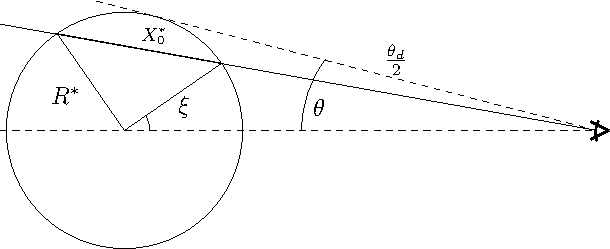
\includegraphics[width=0.7\textwidth]{C:/Users/henri/OneDrive/Documents/NTNU/Semester 10/Masteroppgave/Plots/Radiative_transfer_SSA.pdf}
    \caption{Schematic view of the radiative transfer in a spherical ball of plasma. Image inspired by image from \cite{Hirotani_2005}}
    \label{fig:Radiative_transfer}
\end{figure}

\subsection{Deviation from SSA and Equipartition}
If one calculates the magnetic field using both SSA and Equipartition one expects to not get the exact same results, but given a big discrepancy one cannot assume all the fault lies in only the measurements. In \cite{10.1093/mnras/stt2217}, who used SSA and equipartition calculations for a small sample of CSOs, they also found a discrepancy between the two methods. The SSA had a significantly higher value for the magnetic field. This they argue can, and the weight is on can here, be induced by a free-free absorption effect in the source. Free-free absorption is the absorption of radiation by an electron who is in proximity to an ion. The absorption is a result of the electron being accelerated by the ion and the radiation emitted by the electron is absorbed by the ion. The effect of free-free absorption would shift the spectral peak in SSA to a higher frequency and thus give a higher magnetic field strength in our calculations. This would be a good indicator that the source is harboring ions, which one needs for UHECRs acceleration.

\section{Time-scales analysis}
\label{sec:time_scales}

In order to probe what type of sources could be responsible for the observed UHECRs and neutrinos one can use the relevant time-scales as a measure. The timescales of a source will act as an indicator of the dominant processes in the source and give us an upper boundary for what we could expect of escaping particles. The dominant timescales of a source will be source specific, so further on we will be looking at the timescales of a typical compact AGN. The relevant timescales are the acceleration timescale, the synchrotron cooling timescale, the dynamical timescale, and the photo-pion cooling timescale.

\textbf{Acceleration timescale:}
One starts by determining the acceleration timescale of a proton undergoing first-order Fermi acceleration, the acceleration mechanisms explained in section \ref{sec:acceleration_mechanisms}. The acceleration timescale is given by the equation
\begin{equation}
    t_{acc} =  \frac{\eta \epsilon}{Z e B c}
\end{equation}
Where $\eta$ is the efficiency of the acceleration process with the most efficient acceleration harboring the value $\eta \approx (1-10)$, $\epsilon$ is the energy of the particle, $Z$ is the charge of the particle, $e$ is the elementary charge, $B$ is the magnetic field strength and $c$ is the speed of light. 
Usually the value of $\eta$ is taken to be 1, which is the most efficient acceleration process.

\textbf{Size estimation/ dynamical timescale:}
\label{sec:size_estimation}

The dynamical timescale is a limit on the source's size and can be estimated several ways. The source's size is important since in order to accelerate particles the source must also be able to contain particles. If one does not have good measurements on the source size, but has good fluence measurements of an attributing light curve, one can estimate the size of the source via the variability. From the variability timescale $t_{var}$ one can estimate the size of the source as

\begin{equation}
    R = \frac{c \Gamma t_{var}}{1+z}
\end{equation}

Another way of estimating the source's size is through telescope measurements. For radio sources, one can achieve sufficient accuracy in measurements to estimate the size of the source. If one has the full width at half maximum of an emitting sphere, one can relate this to the total angular size of a spherical source according to \cite{1983ApJ...264..296M} as $\theta = \theta_{\text{FWHM}} 1.8$. If one then knows the distance to the source one can get the physical/linear size of the source as

\begin{equation}
    D_{\text{size}} = \left(\theta_{\text{FWHM}}1.8 \right) \cdot D_A(z)
\end{equation}

Where $D_A(z)$ is the angular diameter distance to the source at its redshift $z$.

A third method of estimating the size of specifically the radius of our radio lobes is outlined in \cite{W_jtowicz_2020}. They use a relation between the total linear size of an object and the estimated relations between the semi-major axis and the semi-minor axis. The argument is that some AGN which are important for this report have relatively large aspect ratios between their axes, with an estimation equaling $b/a \approx 0.25$. From this, they introduce the effective radius of the radio lobes via

\begin{equation}
    R_{\text{lobe}} = \sqrt[3]{ab^2\frac{3}{4}} \approx 0.18 \times LS = 0.18 \times 2 \times a 
\end{equation}


\textbf{Cooling timescales:}

In the source of AGN there will be an environment of magnetic fields and photon fields that will interact with the particles. An important timescale to consider given this environment is often the synchrotron cooling timescale. This is the timescale for a particle to lose energy due to synchrotron radiation. One will have both synchrotron losses for proton and for electrons, but since one is concerned about UHECRs one will focus on protons. The synchrotron cooling timescale for protons is given by the equation

\begin{equation}
    t_{sync} = \frac{6\pi m_p^4 c^3}{\sigma_T m_e^2 B^2 E}.
\end{equation}

Here, $m_p$ is the proton mass, $m_e$ is the electron mass, $\sigma_T$ is the Thomson cross-section, $B$ is the magnetic field strength, $E$ is the energy of the particle, and $c$ is the speed of light.

The last timescale used in this analysis is the pion production timescale. Due to the photon fields a proton will inhabit while accelerating, one needs to consider the pion production timescale. This is the timescale for a proton to interact with a photon and produce a pion. The equation is given by
\begin{equation}
    t_{p\gamma}^{-1}(\varepsilon_p) = \frac{c}{2\gamma_p^2} \int_{\varepsilon_{th}}^{\infty} d\varepsilon \sigma_{pr}(\varepsilon) k_p(\varepsilon) \int_{\varepsilon/2\gamma_p}^{\infty} d\varepsilon' \varepsilon'^{-2} \frac{dn}{d\varepsilon'}
\end{equation}
where $\varepsilon_p$ is the energy of the proton, $\gamma_p$ is the Lorentz factor of the proton, $\varepsilon_{th}$ is the threshold energy for the interaction, $\sigma_{pr}$ is the cross-section for the interaction, $k_p$ is the photon field, and $dn/d\varepsilon$ is the differential photon density.

In our analysis one will follow \cite{BHradiation} to set up the pion resonance timescale. $\sigma_{pr}$, or the cross-section for the interaction is given by a two-step function, and is given as

\begin{equation}
    \sigma(E) = 
    \begin{cases} 
    340 \mu b, \text{cm}^{-2} & \text{if } 390 m_e c^2 < E < 980 m_e c^2 \\
    120 \mu b \, \text{cm}^{-2} & \text{if } E > 980 m_e c^2 
    \end{cases}
\end{equation}

Additionally, the inelasticity of the interaction, or how much energy is lost per interaction, is given as

\begin{equation}
    K(E) = 
    \begin{cases} 
    0.2 & \text{if } 390 m_e c^2 < E < 980 m_e c^2 \\
    0.6 & \text{if } E > 980 m_e c^2 \\
    \end{cases}
\end{equation}

%\begin{figure}
%    \centering
%    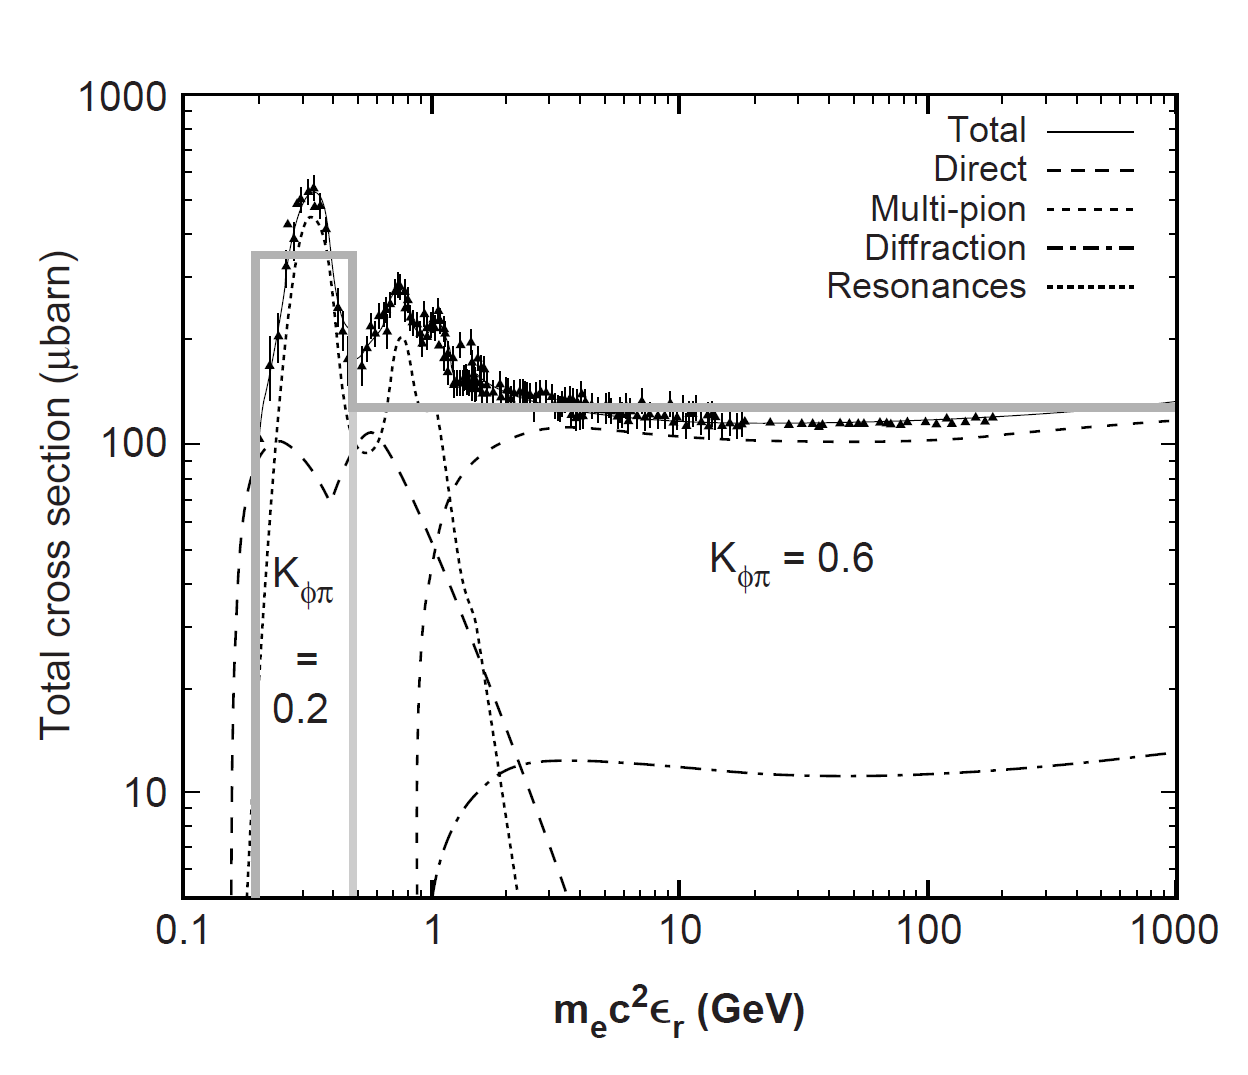
\includegraphics[width=0.5\textwidth]{C:/Users/henri/OneDrive/Documents/NTNU/Semester 10/Masteroppgave/Plots/Dermer_pion_res.png}
%    \caption{Pion resonance cross-section, and the inelasticity of the interaction. Image taken from \cite{BHradiation}}
%    \label{fig:pion_res}
%\end{figure}

%A schematic view of the pion resonance cross-section and the inelasticity of the interaction is shown in Figure \ref{fig:pion_res}. 

The last important parameter in the pion production timescale is the photon field, and one will be using a photon field as described in section \ref{sec:photon_fields}. The specific photon fields will be determined by what source one is looking at and will be clarified in due time.
